
Poly(amido amine) (PAMAM) dendrimer is defined as the dendrimers built using an ethylene-diamine core, a tertiary amine intermediary and a primary amine terminal.
The building blocks are illustrated in Figure \ref{fig:PAMAMBB}.

\begin{figure}
    \centering
    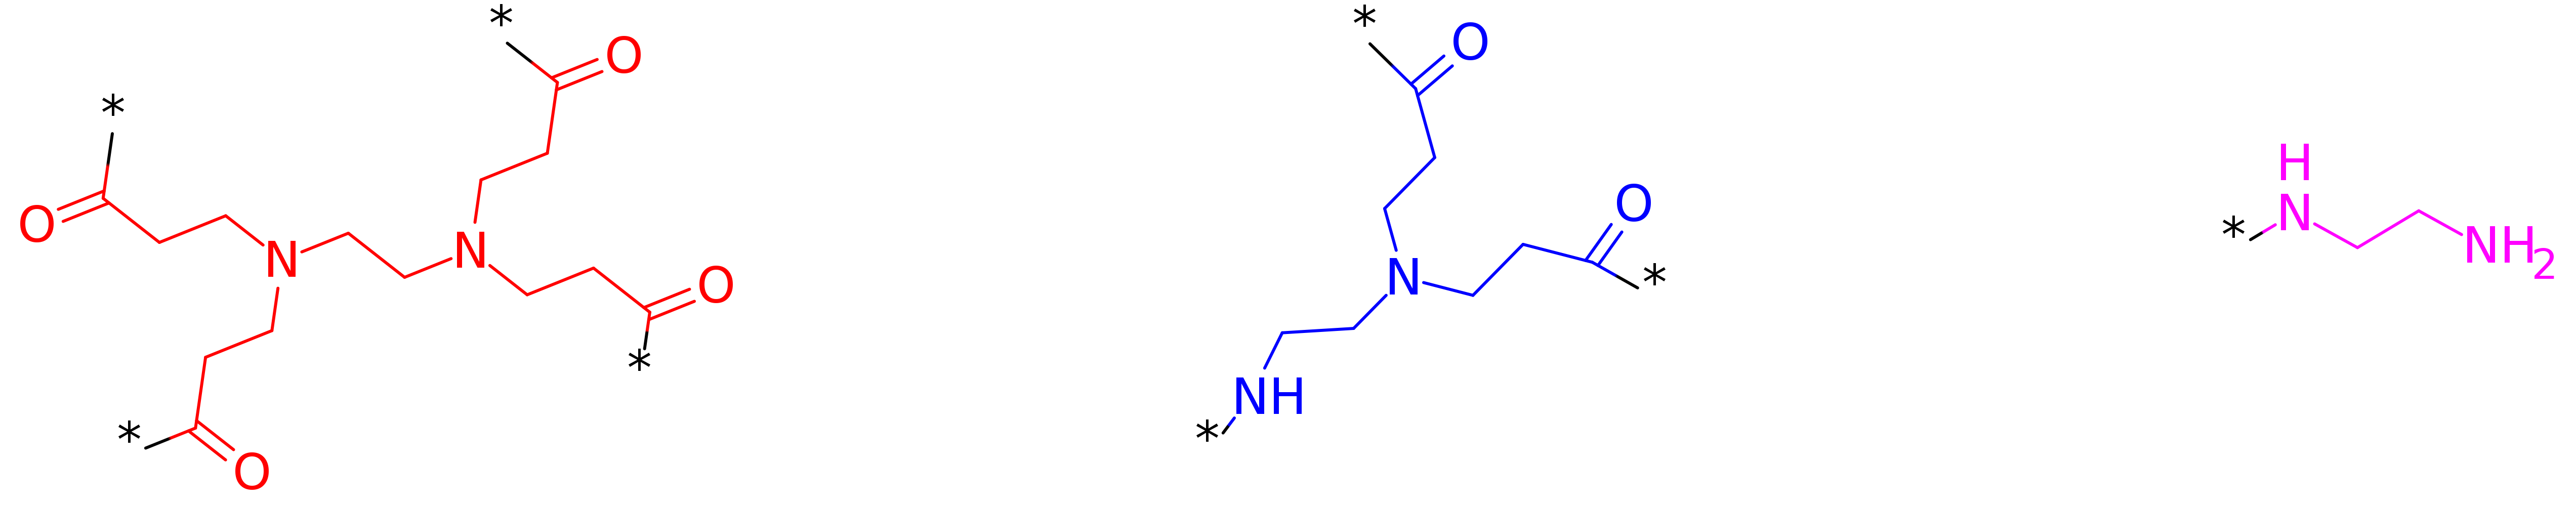
\includegraphics[width=\textwidth]{PAMAM/PAMAMBBs.png}
    \caption{PAMAM dendrimer BBs.
             The core ethylene diamine block is illustrated in red, the intermediary tertiary amine one in blue, and the terminal primary amine block is displayed in pink.}
    \label{fig:PAMAMBB}
\end{figure}

The BBs are provided in the demo directory in pypolybuilder root, whose structure is illustrated below:
\begin{lstlisting}
<path/to/pypolybuilder>/demo/gromacs_format/dendrimer/PAMAM
\end{lstlisting}
\dirtree{%
.1 PAMAM.
.2 core\_PAMAM.itp.
.2 inter\_PAMAM.itp.
.2 ter\_PAMAM.itp.
.2 list\_param.itp.
.2 run.
.3 PAMAM.sh.
.3 PAMAM.top.
.3 mdp.
}

The file names are self-explanatory, the core\_PAMAM.itp file is the MTF for the core block, the inter\_PAMAM.itp for the intermediary, and the ter\_PAMAM.itp, the terminal one.
Once the BBs and the parameters list are successfully built, one can easily run pypolybuilder by using the code line below (also available in file \texttt{how\_to\_run\_this\_example.txt} in demo directory) to obtain a generation 2 PAMAM dendrimer (Figure \ref{fig:PAMAMG2}):

\begin{lstlisting}
python3 ../../../../__main__.py \ --core=core_PAMAM.itp \
--inter=inter_PAMAM.itp \
--ter=ter_PAMAM.itp \
--params=list_param.itp \
--ngen=2 \
--name=PAMAM \
--output=PAMAM.itp \
--gro=PAMAM.gro \
--gromacs \
--dendrimer
\end{lstlisting}

\begin{figure}
    \centering
    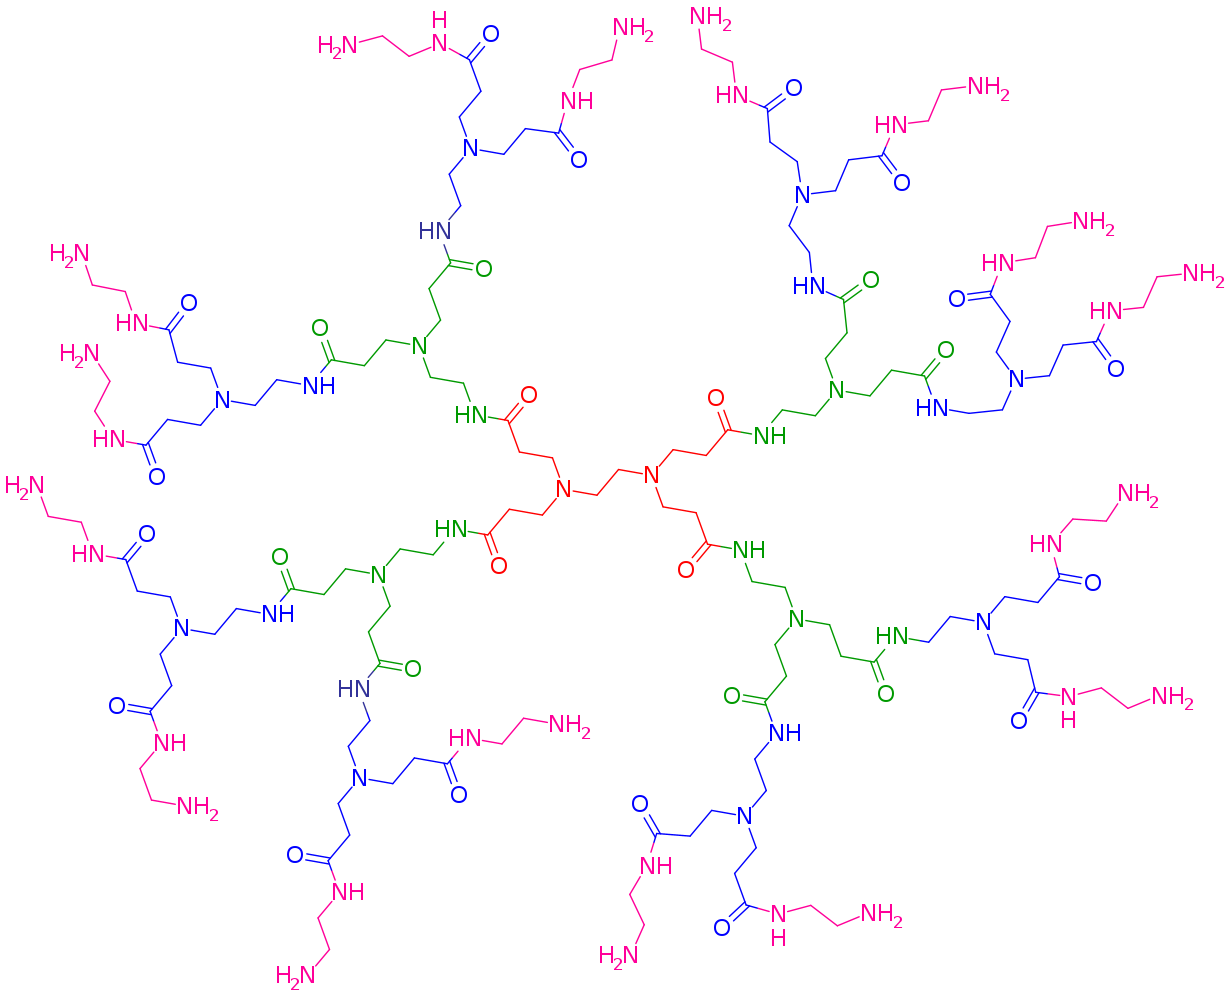
\includegraphics[width=0.5\textwidth]{PAMAM/PAMAMG2.png}
    \caption{PAMAM G2 dendrimer. The color code is the same as the BBs illustrated in Figure \ref{fig:PAMAMBB}. Besides, the first intermediary shell is displayed in green.}
    \label{fig:PAMAMG2}
\end{figure}

The used options in this command line were chosen to select each building block (\texttt{--core}, \texttt{--inter} and \texttt{--ter}), the desired dendrimer generation \texttt{(--ngen}), the name of the topology, for instance the name that will be placed into \texttt{[ moleculetype ]} in the MTF 
(--name), the list of force field parameters for pyPolyBuilder (\texttt{--params}), as well as to name the coordinates and molecular topology output files (\texttt{--gro} and \texttt{--output}, respectively).
Also, the module and the format for the output were selected using, respectively, \texttt{--dendrimer} and \texttt{--gromacs}.

Protonated BBs were also provided and the use of them for creating a protonated PAMAM is left as an exercise.
They have the same file name as the unprotonated BBs but with the suffix ``-protonated''.
Protonated BBs were omitted from the directory tree for simplicity.

After pyPolyBuilder finishes the optimization step, one can use any visualization software to check the output geometry. 
Note that the coordinates are generated considering the molecule in vaccum.
Hence, it may not be the expected solvated conformation (see Figure \ref{fig:PAMAMG2PPB}).
Because of that, the run directory has some scripts to run a short MD simulation in order to equilibrate the molecule in water using gromacs.

\begin{figure}
    \centering
    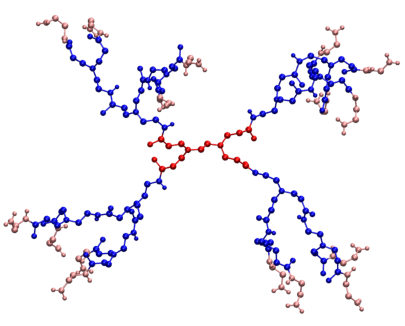
\includegraphics[width=0.5\textwidth]{PAMAM/PAMAM.pdf}
    \caption{Illustration of PAMAM G2 dendrimer generated with pyPolyBuilder.
    The snapshot is displayed in accordance with the previously defined color scheme for the BBs. The core is displayed in red, all intermediary shell monomers are displayed in blue,e and the terminal blocks are in pink.}
    \label{fig:PAMAMG2PPB}
\end{figure}

In order to test the generated MTF and the initial guess for the geometry, we developed an automated script to simulate this tutorial.
PAMAM.sh is a script to automatically solvate, equilibrate and simulate the molecule built in this tutorial.
Even though the simulated time is not long enough to compute properties consistently, it may be used as basis to future simulations and to evaluate the MTF.
%PAMAM.sh is a script to automatically solvate, minimize energy, equilibrate for 100 ps using nvt and npt ensemble and run 100 ps of molecular dynamic simulation (simulation time is far from the desired for this kind of system. However it may be changed in mdp files. Our main goal is to illustrate the generation of a molecular model using pyPolyBuilder).
PAMAM.top is the topology file for the system and mdp  have all required mdp files.
However, these scripts were developed for a specific architecture and should be adapted by the user.
For instance, the path for gromacs needs to be adapted and the output from pyPolyBuilder (PAMAM.gro and PAMAM.itp) needs to be moved to run directory.

After solvation, an energy minization cycle, 100 ps of nvt equilibration, and 100 ps of npt equilibration, the system reaches the conformation illustrated in Figure \ref{fig:PAMAMG2SOL}.

\begin{figure}[ht!]
    \centering
    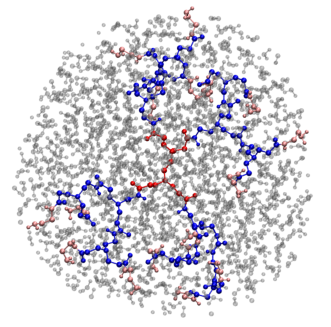
\includegraphics[width=0.5\textwidth]{PAMAM/PAMAMSOL.pdf}
    \caption{Illustration of PAMAM G2 dendrimer. The core is displayed in red, all intermediary shell monomers are displayed in blue, and the terminal blocks are in pink.}
    \label{fig:PAMAMG2SOL}
\end{figure}

A powerful feature of the dendrimer module, is that one can easily generate dendrimers of various sizes by only changing one single integer in the input, the \texttt{--ngen}.
Figure \ref{fig:PAMAMGS} illustrates the procedure of varying \texttt{--ngen} from 0 to 5.

\begin{figure}[ht!]
    \centering
    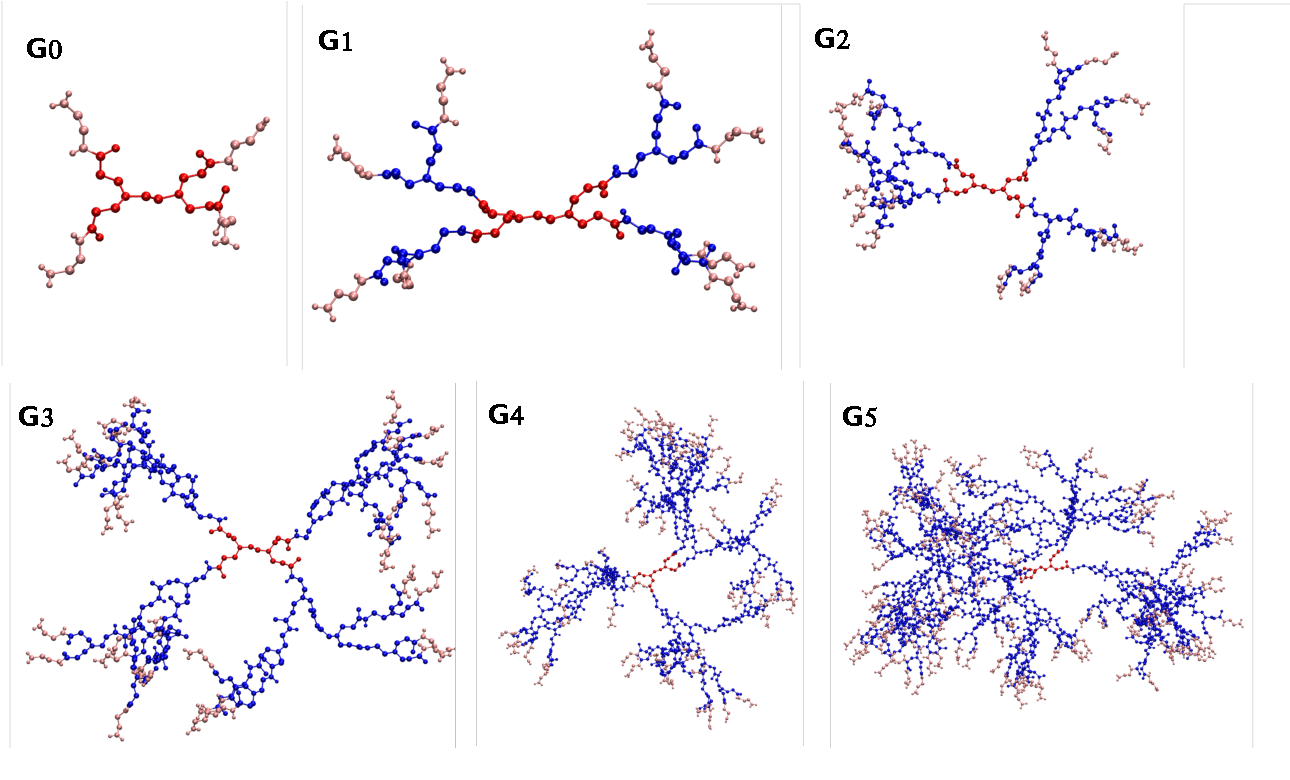
\includegraphics[width=\textwidth]{PAMAM/PAMAMGs.pdf}
    \caption{PAMAM dendrimer from generations 0 to 5 built by using pyPolyBuilder and varying the \texttt{--ngen} option only between each run.
    Color scheme is in accordance with Figure \ref{fig:PAMAMBB}, that is, the core is displayed in red, all shells of intermediary monomers are in blue, and terminal blocks are in pink.}
    \label{fig:PAMAMGS}
\end{figure}